\chapter{Simplifier, multiplier et diviser les nombres fractionnaires}\label{ChSimpMulDivFrac}

\vspace{5cm}
\begin{acquis}
\begin{itemize}
\item 
\item 
\item 
\end{itemize}
\end{acquis}


\activites
\begin{activite}[Q.C.M.]
\begin{enumerate}
\item Parmi les nombres suivants, quelles sont les fractions ?
    \begin{colenumerate}{4}
    \item $\dfrac{3}{11}$
    \item $\dfrac{1,2}{1,7}$
    \item $\dfrac{121}{3}$
    \item $\dfrac{3}{0,8}$
    \end{colenumerate}
\item Quels sont les nombres égaux à $\dfrac{2}{5}$ ?
    \begin{colenumerate}{4}
    \item $2,5$
    \item $0,4$
    \item $\dfrac{6}{15}$
    \item $\dfrac{24}{54}$
    \end{colenumerate}
\item Quelles sont les fractions que l'on ne peut plus simplifier ?
    \begin{colenumerate}{4}
    \item $\dfrac{2}{7}$
    \item $\dfrac{120}{55}$
    \item $\dfrac{99}{117}$
    \item$\dfrac{33}{100}$
    \end{colenumerate}
\item  Quels sont les nombres supérieurs à $\dfrac{19}{9}$ ?
    \begin{colenumerate}{4}
    \item $\dfrac{19}{8}$
    \item $\dfrac{22}{9}$
    \item 2
    \item 3
    \end{colenumerate}
\item  Quelle est la somme de $\dfrac{1}{7}$ et $\dfrac{1}{14}$ ?
    \begin{colenumerate}{4}
    \item $\dfrac{11}{714}$
    \item $\dfrac{2}{21}$
    \item $\dfrac{3}{14}$
    \item $\dfrac{3}{7}$
    \end{colenumerate}
\item  Quel est le produit de $\dfrac{8}{9}$ par $\dfrac{3}{4}$ ?
    \begin{colenumerate}{4}
    \item $\dfrac{24}{36}$
    \item $\dfrac{2}{3}$
    \item $\dfrac{32}{27}$
    \item $\dfrac{32 \times 27}{36}$
    \end{colenumerate}
\end{enumerate}
\end{activite}




\begin{activite}[Signes de quotients]
\begin{enumerate}
\item \begin{enumerate}
    \item Calcule les quotients : $(-3) \div 4$ ; $3 \div (-4)$ et $-(3 \div 4)$.
    \item Qu'en déduis-tu pour les nombres $\dfrac{-3}{4}$ ; $\dfrac{3}{-4}$ et $-\dfrac{3}{4}$ ?
\end{enumerate}
\item De la même façon, que dire des nombres $\dfrac{-2,5}{-3,2}$ ; $\dfrac{2,5}{3,2}$ ; $-\dfrac{-2,5}{3,2}$ ; $-\dfrac{2,5}{-3,2}$ ? Justifie.
\item On veut calculer le produit de $\dfrac{-3}{5}$ par $\dfrac{7}{-8}$.

\vspace{1em}
\textbf{1\up{ère} méthode : on détermine d'abord le signe de ce produit.}

    \begin{enumerate}
        \item  Détermine le signe de chacun des deux nombres. Puis déduis, à l'aide de la règle des signes, le signe du produit des deux nombres.
        \item Termine le calcul.
    \end{enumerate}
    
\vspace{1em}
\textbf{2\up{e} méthode : on applique la règle de la multiplication de deux fractions.}
    \begin{enumerate}
        \item Sachant que $\dfrac{-3}{5} \times \dfrac{7}{-8} = \dfrac{(-3)\times 7}{5 \times (-8)}$, calcule le numérateur et le dénominateur du quotient.
        \item Termine le calcul.
    \end{enumerate}
\end{enumerate}
\end{activite}

%%%%%%%%%%%%%%%%%%%%%%%%%%%%%%%%%%%%%%%%%%%%%%%


\begin{activite}[Produits en croix avec tableur]
\begin{enumerate}
\item Écris trois fractions égales à $\dfrac{3}{5}$ autres que $\dfrac{9}{15}$.

Dans un tableur, remplis les cellules comme ci-dessous :

\begin{center}
    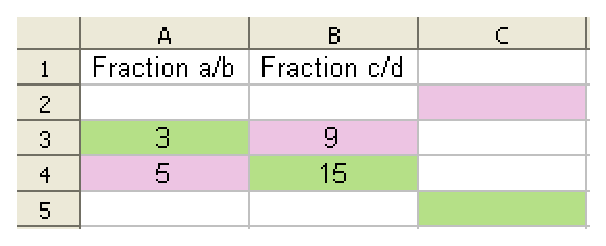
\includegraphics[width=.5\linewidth]{actiTableur}
\end{center}

\item Programme en \texttt{C2} le produit de \texttt{A4} par \texttt{B3} et en \texttt{C5} le produit de \texttt{A3} par \texttt{B4}.
\item Teste dans le tableur les trois fractions trouvées à la question 1. Que remarques-tu dans les cellules \texttt{C2} et \texttt{C5} ?
\item En te servant du tableur, trouve parmi les nombres en écriture fractionnaire suivants ceux qui sont égaux à $\dfrac{3}{5}$ : $\dfrac{301}{501}$ ; $\dfrac{192}{320}$ ; $\dfrac{8,1}{13,5}$ ; $\dfrac{2500}{4000}$.
\item Un nombre en écriture fractionnaire égal à $\dfrac{3}{5}$ s'écrit sous la forme $\dfrac{3\,k}{5\,k}$ où $k$ est un nombre non nul. Démontre que leurs produits en croix sont égaux.
\item On veut déterminer la fraction de dénominateur 120 égale à la fraction $\dfrac{3}{5}$. Remplis les cellules du tableur que l'on connaît et programme en \texttt{B3} le nombre cherché.
\item De la même façon, trouve les nombres manquants : $\dfrac{3}{5}=\dfrac{...}{75}$ ; $\dfrac{3}{5}=\dfrac{...}{125}$ ; $\dfrac{3}{5}=\dfrac{...}{0,25}$.
\end{enumerate}
\end{activite}


%%%%%%%%%%%%%%%%%%%%%%%%%%%%%%%%%%%%%%%%%%%%%%%


\begin{activite}[Inverses]
\begin{enumerate}
\item Quelle est la longueur du côté d'un carré d'aire 1 unité d'aire (U.A.) ?
\item On considère plusieurs rectangles qui ont tous la même aire de 1 U.A.. Recopie puis complète le tableau suivant par les nombres qui conviennent :
 
\renewcommand*\tabularxcolumn[1]{>{\centering\arraybackslash}m{#1}}
\renewcommand{\arraystretch}{1.6}
\begin{CLtableau}{\linewidth}{7}{c}
\hline
& Rectangle 1 & Rectangle 2 & Rectangle 3 & Rectangle 4 & Rectangle 5 & Rectangle 6 \\ \hline
Longueur & 2 & & & 3 & & $\dfrac{4}{3}$ \\ \hline
Largeur & & $0,1$ & $0,25$ & & $\dfrac{1}{7}$ & \\ \hline
\end{CLtableau}

    \begin{enumerate}
        \item Que dire de la longueur de ces rectangles ? Et de la largeur ?
        \item Quel lien y a-t-il entre la longueur et la largeur de ces rectangles ?
        
        \textbf{On dit que deux nombres sont inverses l'un de l'autre quand leur produit est égal à 1.}
        
        \item Recopie et complète : les nombres 2 et ... sont inverses l'un de l'autre, ainsi que $0,1$ et ... ; $0,25$ et ... ; 3 et ... ; $\dfrac{1}{7}$ et ... ; $\dfrac{4}{3}$ et ... .
        
        Que peux-tu dire pour le nombre 1 ?
        
        \item Soit $x$ un nombre non nul, quel est l'inverse de $x$ ? Justifie.
        \item Soient $a$ et $b$ deux nombres non nuls, quel est l'inverse de $\dfrac{a}{b}$ ? Justifie.
    \end{enumerate}
 
\end{enumerate}
\end{activite}



%%%%%%%%%%%%%%%%%%%%%%%%%%%%%%%%%%%%%%%%%%%%%%%



\begin{activite}[Comparaison dans tous les cas]

\begin{partie}[Dénominateurs n'ayant pas de diviseur commun autre que 1]
Corentin le lapin et Luce la puce décident de faire une course. Corentin fait des bonds de $\dfrac{1}{3}$ de mètre tandis que Luce fait des bonds de $\dfrac{1}{5}$ de mètre. 

\begin{center}
    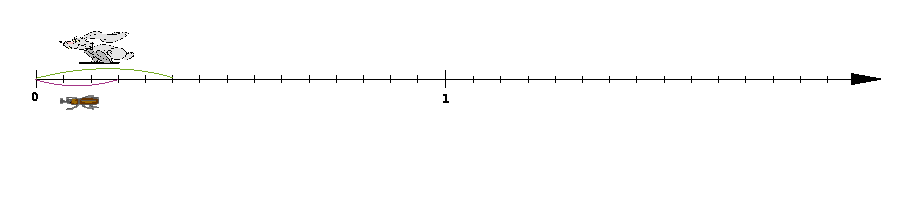
\includegraphics[width=\linewidth]{actiLapinScara}
\end{center}

    \begin{enumerate}
        \item Quand Corentin fait deux bonds, Luce en fait trois. Reproduis la demi-droite graduée ci-dessus représentant la course, puis place les points $C$ et $L$ pour indiquer les positions de Corentin et de Luce.
        \item Complète les phrases suivantes :
        
« Corentin a parcouru $\dfrac{...}{...}$ de mètre, ce qui équivaut à $\dfrac{...}{15}$ de mètre. »

« Luce a parcouru $\dfrac{...}{...}$ de mètre, ce qui équivaut à $\dfrac{...}{15}$ de mètre. »

        \item En t'aidant de la question 2, indique lequel des deux a parcouru la plus grande distance. Parmi les fractions $\dfrac{2}{3}$ et $\dfrac{3}{5}$, laquelle est la plus grande ?
    \end{enumerate}
\end{partie}

\begin{partie}[Dénominateurs ayant plusieurs diviseurs communs]
Lola la tortue et Jeannot le lièvre décident de faire une course sur une demi-droite graduée. Le point de départ est l'origine de la demi-droite. Lola parcourt $\dfrac{5}{4}$ d'unité et Jeannot parcourt $\dfrac{7}{6}$ d'unité.
    \begin{enumerate}
        \item Trace une demi-droite et gradue-la pour y placer les points $L$ et $J$ indiquant les positions de Lola et Jeannot.
        \item Lequel des deux a parcouru le plus grand trajet ? Parmi les fractions $\dfrac{5}{4}$ et $\dfrac{7}{6}$, laquelle est la plus grande ?
    \end{enumerate}
\end{partie}


\begin{partie}[Bilan]
\begin{enumerate}
    \item Énonce une règle qui permet de comparer des fractions de dénominateurs différents.
    \item Applique la règle que tu as trouvée pour comparer : $\dfrac{7}{5}$ et $\dfrac{13}{11}$ puis $\dfrac{3}{25}$ et $\dfrac{1}{10}$.
\end{enumerate}
\end{partie}

\end{activite}

%%%%%%%%%%%%%%%%%%%%%%%%%%%%%%%%%%%%%%%%%%%%%%%


\begin{activite}[Divisions]
\begin{enumerate}
\item Sachant que pour tous nombres $a$ et $b$ non nuls : $\dfrac{a}{b}=a \times \dfrac{1}{b}$, décompose de la même façon le quotient $\dfrac{\dfrac{3}{2}}{\dfrac{5}{3}}$.
\item Que peux-tu dire du nombre $\dfrac{1}{\dfrac{5}{3}}$ ? Déduis-en une fraction égale à ce nombre.
\item Transforme alors le quotient $\dfrac{\dfrac{3}{2}}{\dfrac{5}{3}}$ en produit et complète la phrase suivante : \emph{« Diviser par une fraction, c'est ... .».}
\item Termine alors le calcul du quotient de $\dfrac{3}{2}$ par $\dfrac{5}{3}$.
\item Applique cette règle pour effectuer les calculs suivants : $\dfrac{\dfrac{10}{11}}{\dfrac{7}{8}}$ ; $\dfrac{\dfrac{4}{7}}{\dfrac{5}{9}}$ ; $\dfrac{\dfrac{2}{5}}{\dfrac{14}{3}}$.
\end{enumerate}
\end{activite}


\cours
\section{Amplifier ou réduire un quotient}

\begin{aconnaitre}
\textbf{Si on multiplie ou si on divise} le numérateur et le dénominateur d'un quotient par \textbf{un même nombre non nul} alors on obtient \textbf{quotient égal}.

Pour tous nombres $a$, $b$ et $k$ où $b$ et $k$ sont non nuls :
\[ \frac{a \times k}{b \times k} = \frac{a}{b} \text{ et } \frac{a \div k}{b \div k} = \frac{a}{b}\]
\end{aconnaitre}

\begin{exemple*1}
Simplifie le quotient $\dfrac{42}{-140}$.
\correction

\begin{tabular}{lll}
$\dfrac{42}{-140}=-\dfrac{42}{140}$ & $\longrightarrow$ & On détermine le signe du quotient. \\
$\dfrac{42}{-140}=-\dfrac{3 \times 2 \times 7}{10 \times 7 \times 2}$  & $\longrightarrow$ & On cherche les facteurs communs à 2 et 140. \\
$\dfrac{42}{-140}=-\dfrac{3}{10}$ & $\longrightarrow$ & On simplifie le quotient. \\
\end{tabular}
\end{exemple*1}

\begin{exemple*1}
Détermine le nombre manquant dans l'égalité $\dfrac{-1,2}{6}=\dfrac{...}{18}$.
\correction

\vspace{.5em}
\begin{tabular}{lll}
\hspace{1.5em}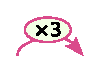
\includegraphics[width=.8cm]{figX3} & & \\
$\dfrac{-1,2}{6}=\dfrac{...}{18}$ & $\longrightarrow$ & Pour passer de 6 à 18 \textbf{on multiplie par 3}. \\
\hspace{1.5em}
\includegraphics[width=.8cm]{figX3b} & & \\
donc $\dfrac{-1,2}{6}=\dfrac{-3,6}{18}$  & $\longrightarrow$ & Ainsi, pour trouver le nombre manquant, \textbf{on multiplie} \\
& & \textbf{$\mathbf{-1,2}$ par 3}, ce qui donne $-3,6$. \\
\end{tabular}
\end{exemple*1}


\section{Comparer deux fractions}

\begin{aconnaitre}[Fractions dont le numérateur et le dénominateur sont positifs]
\begin{itemize}
\item Si les deux fractions ont le même dénominateur, la plus grande est celle qui a le plus grand numérateur.

Par exemple $\dfrac{5}{7}>\dfrac{2}{7}$ car $5 > 2$.

\item Si les deux fractions ont le même numérateur, la plus grande est celle qui a le plus petit dénominateur.

Par exemple $\dfrac{4}{9}<\dfrac{4}{5}$ car $9 > 5$.

\item Si une fraction est plus grande que 1 (son numérateur est plus grand que son dénominateur), alors elle est plus grande qu'une fraction qui est plus petite que 1 (dont le numérateur est plus petit que le dénominateur).

Par exemple $\dfrac{9}{5}>\dfrac{6}{7}$ car $\dfrac{9}{5}>1$ et $\dfrac{6}{7}<1$. 
\end{itemize}
\end{aconnaitre}



\begin{remarque}
Attention, les règles données ci-dessus ne sont pas vraies si le numérateur ou le dénominateur d'une des fractions est négatif.
\end{remarque}

\section{Multiplication}

\begin{aconnaitre}
Pour \textbf{multiplier des nombres en écriture fractionnaire}, on multiplie les numérateurs entre eux et les dénominateurs entre eux.

Pour tous nombres $a$, $b$, $c$ et $d$ où $b$ et $d$ sont non nuls :
\[ \dfrac{a}{b} \times \dfrac{c}{d} = \dfrac{a\times c}{b \times d} \]
\end{aconnaitre}

\begin{remarque}
Si $b=1$, la formule devient $a \times \dfrac{c}{d} = \dfrac{a\times c}{d}$
\end{remarque}

\begin{exemple*1}
Calcule l'expression $B=-\dfrac{35}{33} \times \dfrac{-39}{-80}$. Donne le résultat sous forme simplifiée.
\correction
\vspace{.5em}
 
\begin{tabular}{lll}
$B = -\dfrac{35 \times 39}{33 \times 80}$ & $\longrightarrow$ & On détermine le signe du résultat. \\
$B = -\dfrac{7 \times \mathbf{5} \times 13 \times \mathbf{3}}{11 \times \mathbf{3} \times 2 \times \mathbf{5} \times 8}$ & $\longrightarrow$ & On cherche des facteurs communs. \\
$B = -\dfrac{7 \times 13}{11 \times 2 \times 8}$ & $\longrightarrow$ & On simplifie. \\
$B = -\dfrac{91}{176}$ & $\longrightarrow$ & On calcule. \\
\end{tabular}
\end{exemple*1}

\section{Division de deux quotients}

\subsection{Inversion d'un nombre non nul}

\begin{definition}
\textbf{Deux nombres sont \MotDefinition{inverses}{}} l'un de l'autre si leur produit est égal à 1.
\end{definition}

\begin{propriete}
\begin{itemize}
    \item Tout nombre $x$ non nul admet un inverse qui est le nombre $\dfrac{1}{x}$.
    \item Tout nombre en écriture fractionnaire $\dfrac{a}{b}$ ($a\neq 0$ et $b \neq 0$) admet un inverse qui est le nombre $\dfrac{b}{a}$.
\end{itemize}
\end{propriete}

\begin{remarque}
\begin{itemize}
    \item Un nombre et son inverse ont toujours le même signe.
    
    En effet, leur produit 1 est positif et seul le produit de deux nombres de même signe est positif.
    \item Zéro est le seul nombre qui n'admet pas d'inverse.
    
    En effet, tout nombre multiplié par 0 donne 0 et ne donnera jamais 1.
\end{itemize}
\end{remarque}

\begin{exemple}
Calcule l'inverse de 3.
\correction
L'inverse de 3 est $\dfrac{1}{3}$.
\end{exemple}

\begin{exemple}
Calcule l'inverse de $\dfrac{-7}{3}$.
\correction
L'inverse de $\dfrac{-7}{3}$ est $\dfrac{1}{\dfrac{-7}{3}}=\dfrac{3}{-7}=\dfrac{-3}{7}$.
\end{exemple}

\subsection{Diviser des quotients}

\begin{aconnaitre}
\textbf{Diviser par un nombre non nul} revient à multiplier par l'inverse de ce nombre.

Pour tous nombres $a$, $b$, $c$ et $d$ où $b$, $c$ et $d$ sont non nuls :
\[ \dfrac{a}{b} \div \dfrac{c}{d} = \dfrac{a}{b} \times \dfrac{d}{c} \text{ ou } \dfrac{\phantom{i}\dfrac{a}{b}\phantom{i}}{\dfrac{c}{d}}=\dfrac{a}{b} \times \dfrac{d}{c} \]
\end{aconnaitre}

\begin{exemple*1}
Calcule $C=\dfrac{-8}{7} \div \dfrac{5}{-3}$.
\correction
\vspace{.5em}
 
\begin{tabular}{lll}
$C=+\left(\dfrac{8}{7} \div \dfrac{5}{3}\right)$ & $\longrightarrow$ & On détermine le signe du résultat. \\
$C=\dfrac{8}{7} \times \dfrac{3}{5}$ & $\longrightarrow$ & On multiplie par l'inverse du deuxième quotient. \\
$C=\dfrac{8\times 3}{7\times 5}$ & $\longrightarrow$ & On multiplie les fractions. \\
$C=\dfrac{24}{35}$ & $\longrightarrow$ & On calcule. \\
\end{tabular}
\end{exemple*1}


\begin{exemple*1}
Calcule $D=\dfrac{-\dfrac{32}{21}}{\dfrac{-48}{-35}}$ et donne le résultat en le simplifiant le plus possible.
\correction
\vspace{.5em}
 
\begin{tabular}{lll}
$D=-\dfrac{\dfrac{32}{21}}{\dfrac{48}{35}}$ & $\longrightarrow$ & On détermine le signe du résultat. \\
$D=-\dfrac{32}{21}\times \dfrac{35}{48}$ & $\longrightarrow$ & On multiplie par l'inverse du deuxième quotient. \\
$D=-\dfrac{\mathbf{8}\times \mathbf{2}\times 2 \times \mathbf{7} \times 5}{\mathbf{7 \times 3 \times 3 \times \mathbf{2} \times \mathbf{8}}}$ & $\longrightarrow$ & On cherche des facteurs communs. \\
$D=-\dfrac{10}{9}$ & $\longrightarrow$ & On calcule sans oublier de simplifier avant ! \\
\end{tabular}
\end{exemple*1}


\begin{exemple*1}
Quelle est la nature du nombre $E$ défini par $E=\dfrac{1+\dfrac{2}{3}}{1-\dfrac{2}{3}}$ ?
\correction
\vspace{.5em}
 
\begin{tabular}{lll}
$E=\dfrac{\dfrac{3}{3}+\dfrac{2}{3}}{\dfrac{3}{3}-\dfrac{2}{3}}=\dfrac{\dfrac{5}{3}}{\dfrac{1}{3}}$ & $\longrightarrow$ & $E$ peut s'écrire aussi $E=\left(1+\dfrac{2}{3}\right) \div \left(1-\dfrac{2}{3}\right)$. \\
 & & On commence donc par calculer les parenthèses.\\
$E=\dfrac{5}{3} \times \dfrac{3}{1}$ & $\longrightarrow$ & On multiplie par l'inverse du deuxième quotient. \\
$E=\dfrac{5\times \mathbf{3}}{\mathbf{3}\times 1}$ & $\longrightarrow$ & On cherche des facteurs communs. \\
$E=5$ donc $E$ est un nombre entier. & &  \\
\end{tabular}
\end{exemple*1}


\section{Signe d'une fraction}

\begin{propriete}
Pour déterminer le signe d'une fraction, on utilise la règle du produit des signes.
\end{propriete}

\begin{aconnaitre}
Si une fraction est négative, on peut l'écrire de trois manières différentes en mettant le signe moins au numérateur, au dénominateur (peu utilisé) ou devant la fraction.
On écrira donc indifféremment  $\dfrac{-2}{3}$ ou $-\dfrac{2}{3}$ et rarement $\dfrac{2}{-3}$.
\end{aconnaitre}



\exercicesbase
\begin{colonne*exercice}
\serie{Comparaison}


\begin{exercice}[Signes]
Donne le signe des nombres suivants :

$\dfrac{-5,2}{4,23}$ ; $\dfrac{5}{-2,1}$ ; $\dfrac{472}{23}$ ; $\dfrac{-8,9}{-45}$ ; $-\dfrac{12}{13}$ ; $-\dfrac{11}{-5,2}$.
\end{exercice}





\begin{exercice}
Indique les nombres égaux parmi ceux de la liste ci-dessous :

$\dfrac{-8}{9}$ ; $-\dfrac{8}{9}$ ; $\dfrac{-8}{-9}$ ; $-\dfrac{8}{-9}$ ; $\dfrac{8}{-9}$ ; $-\dfrac{-8}{9}$ ; $\dfrac{8}{9}$.
\end{exercice}




\begin{exercice}[Encadrement]

\begin{enumerate}
\item On considère la fraction $\dfrac{56}{21}$.

Effectue la division euclidienne de 56 par 21 et déduis-en un encadrement de la fraction par deux nombres entiers consécutifs.
\item Encadre $\dfrac{-89}{15}$ puis $\dfrac{47}{59}$ par deux nombres entiers consécutifs.
\item Encadre respectivement $\dfrac{-47}{25}$ et $\dfrac{13}{-4}$ par deux nombres entiers consécutifs et déduis-en la comparaison de ces deux fractions.
\item Peux-tu appliquer la même méthode pour comparer $\dfrac{25}{3}$ et $\dfrac{90}{11}$ ?
\end{enumerate}
\end{exercice}




\begin{exercice}[Avec des valeurs approchées]
Soient deux nombres : $a =\dfrac{816}{577}$  et $b =\dfrac{577}{408}$.
\begin{enumerate}
\item Donne la valeur arrondie de $a$ et celle de $b$ au millième. Peux-tu en déduire la comparaison de $a$ et de $b$ ?
\item Donne des valeurs approchées de $a$ et $b$ qui permettent de les comparer. Compare $a$ et $b$.
\end{enumerate}
\end{exercice}





\begin{exercice}[Égalités]
Recopie et complète chacune des égalités suivantes :
\begin{enumerate}
\item $\dfrac{...}{-5}=\dfrac{10}{20}$
\item $\dfrac{2}{3}=\dfrac{...}{27}$
\item $\dfrac{-15}{45}=\dfrac{-5}{...}$
\item $\dfrac{...}{-18}=\dfrac{7}{6}$
\item $3=\dfrac{...}{4}$
\item $-2,1=-\dfrac{21}{...}$
\end{enumerate}
\end{exercice}




\begin{exercice}
Dans chaque cas, à partir des égalités données et en utilisant seulement les quatre nombres qui apparaissent, écris toutes les égalités d'écritures fractionnaires possibles :
\begin{enumerate}
\item $7 \times (-8) = -4 \times 14$
\item $-3 \times (-1) = 2 \times 1,5$
\item $2,1 \times 12 = 9 \times 2,8$
\item $-4 \times 9 = 12 \times (-3)$
\end{enumerate}
\end{exercice}




\begin{exercice}[Égalité ?]
Recopie et complète en utilisant $=$ ou $\neq$, en justifiant dans chaque cas :
\begin{enumerate}
\item $\dfrac{9}{5} ... \dfrac{26}{15}$ 
\item $\dfrac{-7}{-3} ... \dfrac{-14}{6}$
\item $\dfrac{-12,7}{-5} ... \dfrac{25,4}{10}$
\item $\dfrac{-27,35}{27,35} ... \dfrac{15,72}{-15,72}$
\end{enumerate}
\end{exercice}





\begin{exercice}[Avec un dénominateur entier positif]
Réécris chacune des écritures fractionnaires suivantes avec un dénominateur entier positif :
$\dfrac{4}{-5}$ ; $\dfrac{-8}{-7}$ ; $-\dfrac{5,2}{-7}$ ; $\dfrac{7}{-2,1}$ ; $\dfrac{8,2}{0,12}$ ; $-\dfrac{-1}{-3,54}$.
\end{exercice}





\begin{exercice}[Même dénominateur positif]
\begin{enumerate}
\item Recopie et complète la phrase suivante :

« Deux nombres en écriture fractionnaire de même dénominateur positif sont rangés... ».
\item Compare les nombres suivants :

$\dfrac{-7,5}{3}$ et $\dfrac{-7,49}{3}$ ;

$\dfrac{4,05}{2,1}$ et $\dfrac{4,2}{2,1}$ ;

$-\dfrac{0,74}{5}$ et $\dfrac{-0,7309}{5}$ ; 

$\dfrac{8}{-5,23}$ et $\dfrac{-7,9}{5,23}$. 
\end{enumerate}
\end{exercice}





\begin{exercice}[Avec le même numérateur]
\begin{enumerate}
\item Recopie et complète la phrase suivante :

« Deux nombres positifs en écriture fractionnaire de même numérateur sont rangés… »
\item Compare les nombres suivants :

$\dfrac{3,5}{8,2}$ et $\dfrac{3,5}{8,15}$ ;

$-\dfrac{-1}{6}$ et $\dfrac{1}{5,7}$.
\end{enumerate}
\end{exercice}




\begin{exercice}[Avec le même numérateur (bis)]
Compare les nombres suivants en commençant par comparer leurs opposés :
\begin{enumerate}
\item $\dfrac{1}{-5}$ et $\dfrac{1}{-7}$ ;
\item $\dfrac{-3}{8}$ et $\dfrac{-3}{8,2}$ ;
\item $-\dfrac{5,23}{14,5}$ et $\dfrac{-5,23}{14,6}$ ;
\item $\dfrac{-7,5}{0,23}$ et $\dfrac{75}{-2,4}$. 
\end{enumerate}
\end{exercice}





\begin{exercice}
Dans chaque cas, réécris les nombres avec le même dénominateur positif puis compare-les :
\begin{enumerate} 
\item $\dfrac{-5}{4}$ et $\dfrac{-9}{8}$ ;
\item $\dfrac{2,7}{-9}$ et $\dfrac{-1}{3}$ ;
\item -3 et $-\dfrac{20,9}{-7}$ ;
\item $-\dfrac{2}{11}$ et $\dfrac{-5}{33}$ ; 
\item $\dfrac{7}{2,5}$ et $\dfrac{-20,5}{7,5}$ ; 
\item $\dfrac{13}{-27}$ et $\dfrac{-79}{162}$.
\end{enumerate}
\end{exercice}




\begin{exercice}[Multiple commun]
\begin{enumerate}
\item Quels sont les dix premiers multiples de 12 ? Ceux de 18 ? Déduis-en le plus petit multiple non nul commun à 12 et 18, puis un dénominateur commun positif des fractions : $\dfrac{-7}{12}$ et $\dfrac{-11}{18}$.

Compare alors ces deux nombres.
\item La méthode précédente permet-elle de trouver rapidement un dénominateur commun aux nombres : $\dfrac{8}{11}$ et $\dfrac{10}{13}$ ?

Comment en trouver un alors rapidement ? Compare ces deux nombres.
\end{enumerate}
\end{exercice}





\begin{exercice}Dans chaque cas, réécris les nombres avec le même dénominateur positif, puis compare-les :
\begin{enumerate}
\item $\dfrac{-5}{8}$ et $\dfrac{-3,8}{6}$ ;
\item $\dfrac{14}{5}$ et $\dfrac{20}{7}$ ;
\item $\dfrac{3}{-50}$ et $-\dfrac{4}{75}$ ;
\item $\dfrac{54,5}{0,27}$ et $\dfrac{-2,62}{0,13}$.
\end{enumerate}
\end{exercice}






\begin{exercice}
Compare en justifiant :
\begin{enumerate}
\item $-\dfrac{12}{18}$ et $\dfrac{399}{-300}$ ; 
\item $\dfrac{2}{57}$ et $\dfrac{1}{28,4}$ ;
\item $\dfrac{-75}{47}$ et $\dfrac{25}{-15}$ ;
\item $\dfrac{-5}{6}$ et $-\dfrac{15}{14}$ ;
\item $\dfrac{6}{13}$ et $\dfrac{29}{65}$ ;
\item $\dfrac{3}{-22}$ et $\dfrac{4,5}{33}$.
\end{enumerate}
\end{exercice}




\begin{exercice}[Dans l'ordre]
\begin{enumerate}
\item Range les nombres suivants dans l'ordre croissant sans utiliser de valeurs approchées :

$\dfrac{7}{-15}$ ; $\dfrac{7}{3}$ ; $\dfrac{490}{420}$ ; $\dfrac{-5}{12}$ ; $\dfrac{-24}{-18}$ ; 2,5.
\item Range les nombres suivants dans l'ordre décroissant :

$\dfrac{-29}{100}$ ; $\dfrac{7}{-25}$ ; $-0,285$ ; $-\dfrac{1}{5}$ ; $\dfrac{13}{-50}$ ; 0 ; $\dfrac{-1}{2,5}$.
\end{enumerate}
\end{exercice}





\begin{exercice}[Trajet]
Quatre amis font un voyage en trois jours. Le premier jour, ils parcourent 40\,\%\ du trajet total ; le deuxième jour, un quart et le dernier jour, $\dfrac{7}{20}$ du trajet total.

Quel jour ont-ils parcouru la plus grande distance ?

Peux-tu calculer la distance parcourue chaque jour ?
\end{exercice}







\serie{Multiplications}





\begin{exercice}[La règle et les signes]
Effectue les produits suivants :
\begin{enumerate}
\item $\dfrac{3}{2} \times \dfrac{5}{7}$ ;
\item $\dfrac{-4}{11} \times \dfrac{1}{-3}$ ;
\item $3 \times \dfrac{-7}{5}$ ;
\item $\dfrac{5}{-4} \times \dfrac{5}{-2}$ ;
\item $\dfrac{8}{17} \times \dfrac{5}{-3}$ ;
\item $-\dfrac{13}{5} \times \left(-\dfrac{2}{11}\right)$ ;
\item $\left(-\dfrac{7}{15}\right) \times (-8) \times \dfrac{2}{3}$ ;
\item $\dfrac{-1}{2} \times \dfrac{5}{-4} \times \dfrac{-3}{2}$.
\end{enumerate}
\end{exercice}




\newpage
\begin{exercice}[Toujours plus simple]
Simplifie, si possible, les écritures fractionnaires suivantes :
\begin{enumerate}
\item $\dfrac{-5 \times 2}{2 \times 7}$ ;  
\item $\dfrac{-5 + 2}{7 + 2}$ ;
\item $\dfrac{4 \times (-11)}{4 \times (-11) \times 3}$ ;
\item $\dfrac{8 \times (-3) \times 7 \times 5}{3 \times 5 \times 8 \times 7}$ ;
\item $\dfrac{-5 \times 8}{2 \times (-7)}$ ;
\item $\dfrac{5 \times (-9) \times 2}{(-7) \times 10 \times (-1)}$ ;
\end{enumerate}
\end{exercice}





\begin{exercice}[Calculer en simplifiant]
Pour chacun des produits suivants, applique la règle de multiplication sans effectuer les calculs, simplifie lorsque cela est possible et donne alors le résultat sous la forme d'une fraction irréductible :
\begin{enumerate}
\item $\dfrac{8}{5} \times \dfrac{5}{7}$ ;
\item $\dfrac{-3}{10} \times \dfrac{-11}{3}$ ;
\item $\dfrac{-2}{3} \times \dfrac{-5}{2} \times \dfrac{3}{-7}$ ;
\item $\dfrac{5}{-7} \times \left(-\dfrac{7}{5}\right)$ ;
\item $-15 \times \dfrac{2}{15}$ ;
\item $\left(-\dfrac{8}{3}\right) \times \left(-\dfrac{1}{5}\right) \times 3$.
\end{enumerate}
\end{exercice}




\begin{exercice}Complète les égalités  suivantes :
\begin{enumerate}
\item $\dfrac{8}{...} \times \dfrac{7}{3} = -\dfrac{8}{3}$ ; 
\item $\dfrac{-5}{3} \times \dfrac{7}{...} = \dfrac{7}{6}$ ;
\item $\dfrac{6}{5} \times ... = -6$ ;
\item $\left(-\dfrac{8}{21}\right) \times \dfrac{...}{...} = 1$ ;
\item $\dfrac{...}{10} \times \dfrac{7}{...} = -5$ ;
\item $\dfrac{...}{-9} \times \dfrac{2}{...} = \dfrac{4}{15}$ ;
\item $\dfrac{-5}{...} \times \dfrac{3}{-14} \times \dfrac{...}{25} = \dfrac{-2}{7}$.
\end{enumerate}
\end{exercice}




\begin{exercice}[Simplifier avant de calculer]
\begin{enumerate}
\item Écris 15 sous la forme d'un produit de deux nombres entiers. Décompose de même 20 en produit de nombres entiers positifs les plus petits possibles.
\item Recopie et complète les égalités suivantes :
$\dfrac{15}{7} \times \dfrac{11}{20} = \dfrac{... \times ...}{... \times ...} = \dfrac{(... \times ...) \times ...}{... \times (... \times ... \times ...)}$.
\item Simplifie l'expression obtenue et donne le résultat sous forme d'une fraction irréductible.
\end{enumerate}
\end{exercice}





\begin{exercice}
Calcule les produits suivants en simplifiant, puis donne les résultats sous la forme d'une fraction irréductible :
\begin{enumerate}
\item $\dfrac{-7}{25} \times \dfrac{-5}{8}$ ;
\item $\dfrac{18}{-49} \times \dfrac{14}{27}$ ;
\item $\dfrac{45}{28} \times \dfrac{7}{-15}$ ;
\item $\dfrac{-2}{6} \times \left(-\dfrac{21}{11}\right)$ ;
\item $\dfrac{21}{32} \times \dfrac{108}{49}$ ;
\item $-26 \times \dfrac{-5}{39}$ ;
\item $\dfrac{8}{5} \times \dfrac{-5}{21} \times \left(-\dfrac{9}{16}\right)$ ;
\item $\dfrac{56}{-5} \times \dfrac{30}{21} \dfrac{7}{10}$.
\end{enumerate}
\end{exercice} 




\begin{exercice}[Avec la calculatrice]
Utilise ta calculatrice pour effectuer les produits suivants et donne les résultats sous la forme d'une fraction irréductible :
\begin{enumerate}
\item $\dfrac{686}{-153} \times \dfrac{-99}{-196}$ ; 
\item $\dfrac{2,1}{12,5} \times \left(-\dfrac{6,25}{0,49}\right)$.
\end{enumerate}
\end{exercice}



\begin{exercice}
Calcule mentalement :
\begin{enumerate}
\item les trois quarts de 400 ;
\item le double de $\dfrac{-7}{15}$ ;
\item les cinq septièmes des six cinquièmes de l'unité ;
\item les $\dfrac{7}{10}$ de $\dfrac{9}{10}$.
\end{enumerate}
\end{exercice}




\begin{exercice}[Dépense]
Abdel dépense les $\dfrac{5}{12}$ de son argent de poche, puis les trois quarts de ce qu'il lui reste alors.
\begin{enumerate}
\item Quelle fraction de son argent de poche a-t-il dépensée la deuxième fois ?
\item Le montant de son argent de poche étant de 72\,€, combien a-t-il dépensé au total ?
\end{enumerate}
\end{exercice}


\newpage
\begin{exercice}
Recopie et complète en utilisant $=$ ou $\neq$, en justifiant dans chaque cas :
\begin{enumerate}
\item $\dfrac{-9,1}{5,2} ... \dfrac{79,8}{-45,6}$ ;
\item $\dfrac{-5}{-3} ... \dfrac{-3,5}{2,1}$ ;
\item $\dfrac{17,36}{-22,32} ... -\dfrac{28,7}{36,9}$ ;
\item $\dfrac{-56}{-57} ... \dfrac{57}{58}$ ;
\end{enumerate}
\end{exercice}





\serie{Divisions}


\begin{exercice}Inverses
Recopie et complète les égalités suivantes et écris, dans chaque cas, trois phrases utilisant le mot « inverse(s) » :
\begin{enumerate}
\item $4 \times \dfrac{1}{...} = 1$ ;
\item $... \times 0,25 = 1$ ;
\item $\dfrac{1}{...} \times (-3) = 1$ ;
\item $... \times \left(-\dfrac{1}{15}\right) = 1$ ;
\item $\dfrac{3}{4} \times \dfrac{...}{...} = 1$ ;
\item $\dfrac{...}{-25} \times \dfrac{...}{7} = 1$ ;
\item $... \times \left(-\dfrac{8}{5}\right) = 1$ ;
\item $-0,01 \times ... = 1$
\end{enumerate}
\end{exercice}



\begin{exercice}[Ne pas confondre !]
\begin{enumerate}
\item Recopie et complète les égalités suivantes :
\[ \left(\dfrac{9}{-14}\right) \times ... = 1 et \left(\dfrac{9}{-14}\right) + ... = 0\].
Écris deux phrases, l'une utilisant le mot « opposé(s) » et l'autre, le mot « inverse(s) ».
\item Trouve deux nombres qui sont leur propre inverse. Trouve un nombre qui est son propre opposé.
\item Tous les nombres ont-ils un inverse ? Un opposé ?
\item Quel est l'opposé de l'inverse de 4 ? Quel est l'inverse de l'opposé de 4 ?
\end{enumerate}
\end{exercice}



\begin{exercice}[Inverse]
\begin{enumerate}
\item Recopie et complète le tableau ci-dessous avec des écritures fractionnaires.

\renewcommand*\tabularxcolumn[1]{>{\centering\arraybackslash}m{#1}}
\renewcommand{\arraystretch}{1.6}
\begin{Ctableau}{\linewidth}{7}{c}
\hline
$x$ & 7 & $\dfrac{-3}{5}$ & $-\dfrac{8}{9}$ & $-0,6$ & $1,25$ \\ \hline
$\dfrac{1}{x}$ & & & & & \\ \hline
\end{Ctableau}
\item Détermine l'inverse de l'inverse de chaque nombre. Que remarques-tu ?
\end{enumerate}
\end{exercice}


\begin{exercice}[Mentalement]
\begin{enumerate}
\item Effectue mentalement les calculs suivants : $16 \div 2$ ; $100 \times 0,25$ ; $16 \times 0,5$ ; $100 \div 4$.
\item Justifie les résultats égaux avec la règle de division.
\end{enumerate}
\end{exercice}


\begin{exercice}La règle
Applique dans chaque cas la règle de division puis effectue les calculs :
\begin{enumerate}
\item $\dfrac{2}{3} \div 5$ ; 
\item $\dfrac{-5}{7} \div (-4)$ ;
\item $\dfrac{5}{6} \div \dfrac{7}{-11}$ ;
\item $8 \div \dfrac{1}{8}$ ;
\item $\dfrac{-3}{2} \div \dfrac{-5}{7}$ ;
\item $\dfrac{1}{10} \div \left(-\dfrac{7}{9}\right)$.
\end{enumerate}
\end{exercice}

\begin{exercice}Trait de fraction
Écris les quotients suivants en utilisant le symbole $\div$ puis effectue le calcul :
\[ A = \dfrac{2}{\dfrac{3}{5}}  ; B = \dfrac{\dfrac{2}{3}}{5} ; C = \dfrac{\dfrac{2}{3}}{\dfrac{7}{11}}.\]
\end{exercice}


\begin{exercice}[Division et simplification]
Applique la règle de division, simplifie puis effectue les calculs et donne les résultats sous la forme d'une fraction irréductible :
\begin{enumerate}
\item $\dfrac{8}{-15} \div \dfrac{-4}{5}$ ;
\item $\dfrac{9}{10} \div (-3)$ ;
\item $\dfrac{-4}{45} \div \dfrac{16}{15}$ ;
\item $\dfrac{-5}{6} \div \left(-\dfrac{15}{18}\right)$ ;
\item $12 \div \dfrac{3}{-4}$ ;
\item $1 \div \left(\dfrac{-7}{4}\right)$.
\end{enumerate}
\end{exercice}

\end{colonne*exercice}


\exercicesappr
\begin{colonne*exercice}
%\begin{exercice}[Partage]
\begin{enumerate}
\item Calcule la moitié de $\dfrac{-5}{12}$.
\item Il reste les $\dfrac{7}{8}$ d'un gâteau.

Trois amis décident de se partager équitablement ce reste : quelle fraction du gâteau aura chacun d'entre eux ?
\end{enumerate}
\end{exercice}


\begin{exercice}[Avec des lettres]
\begin{enumerate}
\item Sachant que $a = \dfrac{-2}{21}$  et $b =\dfrac{5}{-7}$, calcule :
\[	\dfrac{a}{b} ; \dfrac{b}{a} ; a \times b ; a + b \text{ et } a - b\]
Tu donneras les résultats sous la forme d'une fraction irréductible.
\item Même consigne avec $a =\dfrac{5}{24}$  et $b =-\dfrac{35}{18}$.
\end{enumerate}
\end{exercice}


\begin{exercice}
Jenny avait 145 fr. Elle a dépensé les $\dfrac{2}{5}$ de ce qu'elle avait. Combien d’argent lui reste-t-il ?
\end{exercice}


\begin{exercice}
Un salarié gagne 3900 CHF par mois. Il dépense $\dfrac{3}{20}$ de cette somme pour son loyer, $\dfrac{1}{13}$ pour les impôts et 2000 CHF pour vivre. Combien économise-t-il chaque mois ?
\end{exercice}

\columnbreak
\begin{exercice}
J'ai dépensé les $\dfrac{4}{5}$ de mon argent pour acheter un livre qui coûtait 32 CHF. Quelle somme avais-je dans mon porte-monnaie?
\end{exercice}


\begin{exercice}
Olivier a les $\dfrac{7}{16}$ des $\dfrac{2}{3}$ de l'âge de sa mère qui a 48 ans. Quel est l’âge d’Olivier ?
\end{exercice}


\begin{exercice}
Pierre dit à sa sœur pour l'impressionner: « Ce livre a coûté très cher. Je l'ai payé $\dfrac{5}{12}$ des $\dfrac{6}{5}$ de 20 CHF. » Quel est le prix du livre ?
\end{exercice}


\begin{exercice}
Alicia et Alizée ont groupé leurs économies pour s’acheter un lecteur MP3 et des DVD. 

Elles ont dépensé les $\dfrac{6}{10}$ de leur pactole pour l'achat du lecteur MP3 et les $\dfrac{6}{9}$ de ce qu'il restait pour l’acquisition des DVD. Après ces achats, il ne leur reste plus que 28 €.
\begin{enumerate}
\item De quelle somme disposaient-elles avant de faire leurs achats ? 
\item Quel est le prix du lecteur MP3 et celui des DVD ?
\end{enumerate}
\end{exercice}


\begin{exercice}
Monsieur Reesh avait 500 000 CHF dans son coffre mais Arsène Lupin est passé par là et lui a dérobé $\dfrac{3}{4}$ des $\dfrac{5}{6}$ des $\dfrac{4}{5}$ de la somme. Combien lui reste-t-il dans son coffre ?
\end{exercice}


\begin{exercice}
Lors de ses dernières vacances, Alex a dépensé les $\dfrac{3}{4}$ des $\dfrac{5}{9}$ des $\dfrac{7}{10}$ de son argent de poche qui se montait à 3000 CHF. Quelle somme lui reste-t-il ?
\end{exercice}


\end{colonne*exercice}

\connaissances
%\QCMautoevaluation{Pour chaque question, plusieurs réponses sont proposées. Déterminer celles qui sont correctes.}

\begin{QCM}
\begin{GroupeQCM}

\begin{exercice}
La valeur arrondie au dixième de $\dfrac{2}{3}$ est...
\begin{ChoixQCM}{4}
\item $0$
\item $1$
\item $0,6$
\item $0,7$
\end{ChoixQCM}
\begin{corrige}
\reponseQCM{a}
\end{corrige}
\end{exercice}

\begin{exercice}
Une valeur approchée de $\dfrac{19}{13}$ au millième près est...
\begin{ChoixQCM}{4}
\item $1,46$
\item $1,461$
\item $1,462$
\item $1,4615$
\end{ChoixQCM}
\begin{corrige}
\reponseQCM{a}
\end{corrige}
\end{exercice}


\begin{exercice}
$\dfrac{-24}{-18}=...$
\begin{ChoixQCM}{4}
\item $\dfrac{20}{15}$
\item $-\dfrac{4}{3}$
\item $1,33$
\item $\dfrac{4}{3}$
\end{ChoixQCM}
\begin{corrige}
\reponseQCM{a}
\end{corrige}
\end{exercice}


\begin{exercice}
L'opposé de $\dfrac{4}{5}$ est...
\begin{ChoixQCM}{4}
\item $\dfrac{5}{4}$
\item $\dfrac{-4}{-5}$
\item $\dfrac{-4}{5}$
\item $-\dfrac{4}{5}$
\end{ChoixQCM}
\begin{corrige}
\reponseQCM{a}
\end{corrige}
\end{exercice}


\begin{exercice}
$\left(\dfrac{4}{5}\right)^{-1} = ...$
\begin{ChoixQCM}{4}
\item $\dfrac{3}{5}$
\item $\dfrac{-4}{-5}$
\item $\dfrac{5}{4}$
\item $-\dfrac{4}{5}$
\end{ChoixQCM}
\begin{corrige}
\reponseQCM{a}
\end{corrige}
\end{exercice}


\end{GroupeQCM}


\begin{GroupeQCM}

\begin{exercice}
$\dfrac{37}{15}$ est supérieur à...
\begin{ChoixQCM}{4}
\item $2$
\item $\dfrac{77}{30}$
\item $\dfrac{598}{599}$
\item $\dfrac{25}{10}$
\end{ChoixQCM}
\begin{corrige}
\reponseQCM{a}
\end{corrige}
\end{exercice}


\begin{exercice}
$\dfrac{-14}{5}$ est inférieur à...
\begin{ChoixQCM}{4}
\item $\dfrac{14}{-5}$
\item $-2$
\item $\dfrac{-14}{3}$
\item son inverse
\end{ChoixQCM}
\begin{corrige}
\reponseQCM{a}
\end{corrige}
\end{exercice}


\begin{exercice}
$\dfrac{-5}{6}$ est le résultat de...
\begin{ChoixQCM}{4}
\item $\dfrac{-1}{3} \times \dfrac{-5}{2}$
\item $\dfrac{-5}{11} \times \dfrac{11}{6}$
\item $\dfrac{-30}{36} \div 6$
\item $-5 \times \dfrac{1}{6}$
\end{ChoixQCM}
\begin{corrige}
\reponseQCM{a}
\end{corrige}
\end{exercice}


\begin{exercice}
$-\dfrac{7}{5} \div \dfrac{2}{-3}=...$
\begin{ChoixQCM}{4}
\item $2,1$
\item $\dfrac{10}{21}$
\item $\dfrac{3,5}{1,6}$
\item $-\dfrac{21}{10}$
\end{ChoixQCM}
\begin{corrige}
\reponseQCM{a}
\end{corrige}
\end{exercice}


\begin{exercice}
$\dfrac{\dfrac{2}{3}}{4}=...$
\begin{ChoixQCM}{4}
\item $2 \div 3 \div 4$
\item $\dfrac{8}{3}$
\item $\dfrac{2}{12}$
\item On ne peut pas calculer
\end{ChoixQCM}
\begin{corrige}
\reponseQCM{a}
\end{corrige}
\end{exercice}

\end{GroupeQCM}
\end{QCM}

\TravauxPratiques
%\begin{TP}[Dominos en fractions]


Vous allez créer un jeu de dominos utilisant des fractions.

\begin{enumerate}
    \item Répartissez-vous le travail pour compléter le tableau ci-dessous. La première ligne (cases A1 à F1) contient les résultats des calculs situés dans les lignes 2 à 7.

\vspace{1em}
\renewcommand*\tabularxcolumn[1]{>{\centering\arraybackslash}m{#1}}
\renewcommand{\arraystretch}{1.6}
\begin{cltableau}{\linewidth}{7}
\hline
 & A & B & C & D & E & F \\ \hline
1 & $\dfrac{5}{3}$ & $\dfrac{-3}{5}$ & $\dfrac{3}{5}$ & $\dfrac{-9}{4}$ & $\dfrac{2}{7}$ & $3$ \\ \hline
2 & $\dfrac{1}{3} + \dfrac{4}{3}$ & $\dfrac{-4}{5} +\dfrac{1}{5}$ & & & & \\ \hline
3 & $\dfrac{7}{3}-\dfrac{4}{6}$ & $\dfrac{2}{15}-\dfrac{1}{5}-\dfrac{8}{15}$ & & & & \\ \hline
4 & $\dfrac{2}{3}+1$ & $\dfrac{12}{5}-3$ & & & & \\ \hline
5 & & & & & & \\ \hline
6 & & & & & & \\ \hline
7 & & & & & & \\ \hline
\end{cltableau}

\vspace{1em}

Quelques exemples (cases A2, B2, A3, B3, A4, B4) ont été donnés à titre indicatif. Pour chaque colonne, il faut trouver :
\begin{itemize}
    \item ligne 2 : une somme algébrique de fractions de même dénominateur ;
    \item ligne 3 : une somme algébrique de fractions de dénominateurs différents ;
    \item ligne 4 : une somme algébrique d'un nombre entier et d'une fraction ;
    \item ligne 5 : un produit de deux fractions ;
    \item ligne 6 : un produit de trois fractions ;
    \item ligne 7 : un quotient de deux fractions.
\end{itemize}

    \item Créez le jeu de dominos en respectant le plan suivant (à chaque fois, il faut remplacer le nom de la case par son contenu).
    
    Taille d'un domino : 6\,cm sur 2\,cm.
    
    \vspace{1em}
    \begin{center}
        \renewcommand*\tabularxcolumn[1]{>{\centering\arraybackslash}m{#1}}
        \begin{tabularx}{.6\linewidth}{|X|X|X|X|X|X|X|X|}
        \cline{1-2} \cline{4-5} \cline{7-8}
            A1 & A2 & & A3 & B1 & & A4 & C2 \\ \cline{1-2} \cline{4-5} \cline{7-8}
        \end{tabularx}
        \vspace{.5em}
        
        \begin{tabularx}{.6\linewidth}{|X|X|X|X|X|X|X|X|}
        \cline{1-2} \cline{4-5} \cline{7-8}
            A5 & D3 & & A6 & E4 & & A7 & F5 \\ \cline{1-2} \cline{4-5} \cline{7-8}
        \end{tabularx}
        \vspace{.5em}
        
        \begin{tabularx}{.6\linewidth}{|X|X|X|X|X|X|X|X|}
        \cline{1-2} \cline{4-5} \cline{7-8}
            B2 & B3 & & B4 & C1 & & B5 & D2 \\ \cline{1-2} \cline{4-5} \cline{7-8}
        \end{tabularx}
        \vspace{.5em}
        
        \begin{tabularx}{.6\linewidth}{|X|X|X|X|X|X|X|X|}
        \cline{1-2} \cline{4-5} \cline{7-8}
            B6 & E3 & & B7 & F4 & & C3 & C4 \\ \cline{1-2} \cline{4-5} \cline{7-8}
        \end{tabularx}
        \vspace{.5em}
        
        \begin{tabularx}{.6\linewidth}{|X|X|X|X|X|X|X|X|}
        \cline{1-2} \cline{4-5} \cline{7-8}
            C5 & D1 & & C6 & E2 & & C7 & F3 \\ \cline{1-2} \cline{4-5} \cline{7-8}
        \end{tabularx}
        \vspace{.5em}
        
        \begin{tabularx}{.6\linewidth}{|X|X|X|X|X|X|X|X|}
        \cline{1-2} \cline{4-5} \cline{7-8}
            D4 & D5 & & D6 & E1 & & D7 & F2 \\ \cline{1-2} \cline{4-5} \cline{7-8}
        \end{tabularx}
        \vspace{.5em}
        
        \begin{tabularx}{.6\linewidth}{|X|X|X|X|X|X|X|X|}
        \cline{1-2} \cline{4-5} \cline{7-8}
            E5 & E6 & & E7 & F1 & & F6 & F7 \\ \cline{1-2} \cline{4-5} \cline{7-8}
        \end{tabularx}
    \end{center}
    
    \item Découpez les dominos et échangez votre jeu avec un autre groupe. Il ne vous reste plus qu'à jouer en accolant deux cases de même valeur.
\end{enumerate}
\end{TP}

\begin{TP}[Fractions en tableur]

\begin{enumerate}
    \item Calculez puis donnez le résultat sous forme d'une fraction la plus simple possible :
    \[ A = \dfrac{-3}{7} \times \dfrac{5}{2} ; \qquad	B = \dfrac{2}{3} \times \dfrac{9}{2} \]
    \[ C = \dfrac{2}{3} + \dfrac{3}{4} ; \qquad    D = \dfrac{5}{6} + \dfrac{3}{8} \]
    \item Vous allez créer un modèle de fichier tableur permettant de trouver le produit de deux fractions :
    
    \begin{center}
        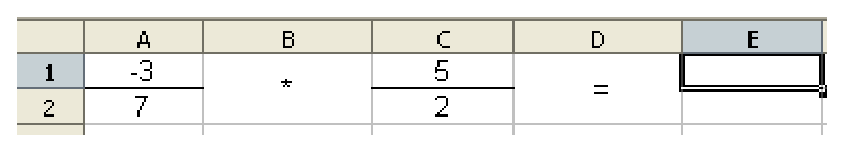
\includegraphics[width=.6\linewidth]{tableur1}
    \end{center}
    
    \begin{itemize}
        \item Recopiez les cellules ci-dessus ;
        \item Dans la cellule E1, tapez « \texttt{=A1*C1} » ;
        \item Dans la cellule E2, tapez « \texttt{=A2*C2} » ;
        \item Utilisez cette feuille de calcul pour vérifier le résultat du calcul B (question a.). Que remarquez-vous ?
    \end{itemize}
    
    \item Sur le même fichier, vous allez maintenant construire un outil permettant de calculer la somme de deux fractions.
    
    \begin{center}
        \includegraphics[width=.6\linewidth]{tableur2}
    \end{center}
    
    Recopiez les cellules ci-dessus ;
    Que faut-il taper comme formules dans les cellules E4 et E5 ?
    Utilisez cette feuille de calcul pour vérifier le résultat du calcul D (question a.). Que remarquez-vous ?
    \item Procédez de la même façon pour construire sur le même fichier quatre outils permettant :
    \begin{itemize}
        \item de calculer le produit de trois fractions ;
        \item de calculer la différence de deux fractions ;
        \item de calculer la somme de trois fractions ;
        \item de calculer le quotient de deux fractions.
    \end{itemize}
    \item Construisez un nouvel outil permettant de calculer la somme de deux fractions en faisant apparaître les étapes intermédiaires.
    \item Refaites tous les calculs avec le fichier tableur qui se trouve en complément. Quelle est la nouveauté apportée par ce fichier par rapport au vôtre ?
    \item Dans quels cas, les deux fichiers donnent-ils des résultats identiques ?
\end{enumerate}
\end{TP}

\recreation % avec R majuscule pour saut de page
%\begin{enigme}[Étourdi !]
Un abreuvoir est alimenté par deux robinets. Lorsque le robinet d'évacuation est fermé, le premier robinet seul le remplit en 4 heures. Le deuxième robinet seul le remplit en 3 heures.

\vspace{.5em}

Lorsque l'abreuvoir est plein, le robinet d'évacuation le vide en 2 heures.

\vspace{.5em}

Alors que l'abreuvoir est vide, l'éleveur ouvre les deux robinets pour le remplir,
mais oublie de fermer le robinet d'évacuation !

\vspace{.5em}

L'abreuvoir va-t-il quand même se remplir ?

Si oui, en combien de temps ?
\end{enigme}



